\documentclass[conference]{IEEEtran}
\usepackage[utf8]{inputenc}
\usepackage[T1]{fontenc}
\usepackage[brazilian]{babel}
\usepackage{amsmath,amssymb,amsfonts}
\usepackage{graphicx}
\usepackage{textcomp}
\usepackage{xcolor}
\usepackage{lmodern}

\begin{document}

\title{Simulador de Escalonamento de Processos}

\author{
\IEEEauthorblockN{Elder Rayan Oliveira Silva}
\IEEEauthorblockA{\textit{UFCA - Universidade Federal do Cariri} \\ @eldrayan}
\and
\IEEEauthorblockN{Espedito Ramom Mascena Ricarto}
\IEEEauthorblockA{\textit{UFCA - Universidade Federal do Cariri} \\ @RamomRicarto}
\and
\IEEEauthorblockN{Manoel Junio Duarte da Silva}
\IEEEauthorblockA{\textit{UFCA - Universidade Federal do Cariri} \\ @Junio404}
\and
\IEEEauthorblockN{Pedro Yan Alcantara Palácio}
\IEEEauthorblockA{\textit{UFCA - Universidade Federal do Cariri} \\ @pedropalacioo}
\and
\IEEEauthorblockN{Sabrina Alencar Soares}
\IEEEauthorblockA{\textit{UFCA - Universidade Federal do Cariri} \\ @sabrinaalencar}
\and
\IEEEauthorblockN{Samuel Wagner Tiburi Silveira}
\IEEEauthorblockA{\textit{UFCA - Universidade Federal do Cariri} \\ @samsilveira}
\and
\IEEEauthorblockN{Sebastião Sousa Soares}
\IEEEauthorblockA{\textit{UFCA - Universidade Federal do Cariri} \\ @SebastiaoSoares}
}

\maketitle\begin{abstract}
Este artigo apresenta o desenvolvimento e a avaliação estatística de um simulador de escalonamento de processos para sistemas operacionais. Foram comparadas três políticas clássicas (FCFS, Round Robin e Prioridade Estática), uma política adaptada (SJF Não-Preemptivo) e uma abordagem própria denominada Prioridade Dinâmica Baseada em Histórico (PDBH). Através da execução de 2.000 cargas de trabalho distribuídas em quatro cenários (Equilibrado, I/O-Bound, CPU-Bound e Desbalanceado), avaliou-se o \textit{trade-off} entre o Tempo de Retorno (\textit{Turnaround}), a Equidade (Índice de Jain) e o custo sistêmico (Trocas de Contexto). Os resultados demonstram o alto nível de inanição em políticas de prioridade estática e os altos custos de troca de contexto do Round Robin. Em relação ao algoritmo proposto (PDBH), os dados revelam que aplicar pontuações dinâmicas de histórico em arquiteturas estritamente não preemptivas não traz benefícios na prática, cenário no qual o algoritmo não obteve ganhos, apresentando resultados equivalentes ao FCFS em todas as métricas observadas.
\end{abstract}

\begin{IEEEkeywords}
Sistemas Operacionais, Escalonamento de Processos, Simulação, Avaliação de Desempenho.
\end{IEEEkeywords}

\section{Introdução}
O escalonamento de processos é uma das funções mais críticas de um Sistema Operacional, responsável por multiplexar o uso do processador (CPU) entre diversas tarefas concorrentes. A escolha da política de escalonamento afeta diretamente o desempenho percebido pelo usuário e a eficiência global do sistema, exigindo um equilíbrio constante entre métricas conflitantes, como a minimização do tempo de espera e a garantia de justiça (equidade) na alocação de recursos.

Políticas clássicas apresentam comportamentos teóricos bem estabelecidos~\cite{silberschatz}: abordagens baseadas em ordem de chegada (FCFS) são simples, mas vulneráveis ao efeito comboio; o fatiamento de tempo (\textit{Round Robin}) promove justiça à custa de frequentes trocas de contexto; e algoritmos baseados em prioridade estática otimizam a execução de tarefas críticas, mas introduzem o risco crônico de inanição (\textit{starvation}) para processos menos favorecidos.

Para analisar essas dinâmicas de forma empírica e reprodutível, este trabalho apresenta o desenvolvimento de um simulador de eventos discretos. Além de implementar os algoritmos clássicos obrigatórios (FCFS, Round Robin, Prioridade Estática e SJF), o projeto propõe e avalia de forma aprofundada a Prioridade Dinâmica Baseada em Histórico (PDBH). Este algoritmo próprio, de natureza não preemptiva, visa mitigar a inanição por meio da aplicação de bônus atrelados ao tempo de espera e penalidades proporcionais ao consumo acumulado de CPU.

Através de um rigoroso protocolo experimental com 2.000 execuções, este artigo avalia o desempenho estrutural e estatístico desses algoritmos sob quatro cenários distintos de carga de trabalho. O objetivo principal é quantificar os \textit{trade-offs} sistêmicos e investigar criticamente o impacto, os custos introduzidos e a eficácia mecânica do algoritmo próprio (PDBH) em comparação às soluções clássicas.

\section{Modelo da Simulação}
Esta seção descreve o modelo arquitetural adotado pelo motor de simulação para representar o comportamento de um sistema operacional monoprocessado.

\subsection{Tempo discreto e eventos}
A simulação é baseada em eventos e controlada por uma unidade de tempo discreta denominada \textit{tick}. O motor avança no tempo processando as transições de estado dos processos.

\subsection{Processos e rajadas}
Cada processo é modelado como uma sequência alternada de rajadas de execução na CPU e requisições de Entrada/Saída (E/S). Os processos chegam ao sistema em instantes de tempo predeterminados e são inseridos na fila de prontos.

\subsection{Modelo de E/S}
Quando um processo solicita uma operação de E/S, ele abandona a CPU e passa para o estado de bloqueio. Ao concluir o tempo necessário para a operação, o processo retorna à fila de prontos, recebendo um novo instante de entrada (\textit{ready\_since}) para fins de desempate e cálculo de espera.

\subsection{Troca de contexto}
A troca de contexto impõe um custo fixo ao sistema. Quando a CPU é repassada para um processo com Identificador de Processo (PID) diferente do que estava em execução anteriormente, adiciona-se o custo de 1 \textit{tick} ao tempo total. O primeiro despacho da simulação não acarreta esse custo.

\subsection{Informações observáveis pelos escalonadores}
Para garantir a ausência de conhecimento futuro, os escalonadores tomam decisões baseadas exclusivamente no estado presente e passado. Nenhuma política tem acesso à duração de rajadas futuras, ao tempo restante de execução ou a informações sobre processos que ainda não chegaram ao sistema.

\section{Algoritmos}
Esta seção detalha os algoritmos de escalonamento implementados.

\subsection{FCFS}
O FCFS (\textit{First-Come, First-Served}) foi implementado como uma política não preemptiva. A fila de prontos é ordenada pelo par $(ready\_since, PID)$: seleciona-se primeiro o processo que está há mais tempo continuamente pronto e, em caso de empate no tempo, o menor PID determina a escolha. Ao retornar de E/S, o processo recebe um novo $ready\_since$ correspondente ao instante da conclusão da operação. A política é consultada apenas quando a CPU está livre; chegadas ou fins de E/S não causam preempção.

\subsection{Round Robin}
O Round Robin (RR) usa uma fila FIFO e um \textit{quantum} padrão de 4 \textit{ticks}. A cada despacho, o contador do \textit{quantum} é reiniciado. Se a rajada de CPU termina antes ou no mesmo \textit{tick} em que o \textit{quantum} se esgota, ocorre a conclusão natural, sem registro de preempção. Quando o \textit{quantum} termina e ainda resta CPU, eventos de fim de E/S e novas chegadas do mesmo \textit{tick} são inseridos primeiro. O processo preemptado recebe um novo $ready\_since$ e é reinserido no fim da fila.

\subsection{Prioridade Não Preemptiva}
Nesta política, valores numéricos menores representam prioridades mais altas (0 a 9). A fila é ordenada pela tupla $(prioridade, ready\_since, PID)$. A prioridade é estática. A política é estritamente não preemptiva: a chegada de um processo mais prioritário não interrompe a rajada em andamento. A reordenação só afeta o próximo despacho.

\subsection{SJF Não-Preemptivo com Estimativa}
O SJF (\textit{Shortest Job First}) clássico foi adaptado para estimar o próximo pico de CPU utilizando uma média móvel exponencial: $\tau_{n+1} = \alpha t_n + (1 - \alpha) \tau_n$, com fator de decaimento $\alpha = 0,5$ e estimativa inicial $\tau_0 = 10,0$. É puramente não preemptivo, priorizando tarefas com a menor estimativa e usando o tempo de chegada para desempate.

\subsection{Algoritmo Proposto: Prioridade Dinâmica Baseada em Histórico (PDBH)}
O PDBH foi desenvolvido como uma iniciativa para mitigar o risco crônico de inanição (\textit{starvation}) da política de Prioridade Estática não preemptiva. O modelo recompensa processos que aguardam muito tempo na fila e penaliza os que monopolizam a CPU, inspirado nos conceitos de envelhecimento (\textit{aging}) e em Filas de Múltiplo Nível com Realimentação.

O PDBH recalcula a prioridade efetiva de cada processo dinamicamente a cada ponto de decisão (despacho). Menores valores numéricos indicam maior prioridade. O cálculo é definido por:

$Score = Prioridade\_Estatica - Bonus\_Espera + Penalidade\_CPU$

Onde o bônus de espera equivale a $\lfloor (Tempo\_Atual - Ready\_Since) / 10 \rfloor$ (1 ponto de melhora a cada 10 \textit{ticks} na fila) e a penalidade por CPU equivale a $\lfloor CPU\_Consumida / 5 \rfloor$ (1 ponto de piora a cada 5 \textit{ticks} processados no total). Empates na pontuação final são resolvidos pelo menor tempo de entrada na fila ($ready\_since$) e, em seguida, pelo menor PID. O algoritmo opera de forma não preemptiva.

\section{Metodologia}
Para garantir a significância estatística, o protocolo experimental contou com 2.000 execuções isoladas. Foram definidos quatro cenários de carga de trabalho obrigatórios:
\begin{itemize}
    \item \textbf{Equilibrado}: Mix proporcional de processos.
    \item \textbf{I/O-Bound}: Tarefas realizam frequentes bloqueios de E/S.
    \item \textbf{CPU-Bound}: Tarefas de longa duração de processamento e pouca E/S.
    \item \textbf{Desbalanceado}: 70\% dos processos são injetados com alta prioridade.
\end{itemize}

Em cada cenário, os cinco algoritmos processaram 100 cargas de trabalho idênticas (1.000 processos cada, gerados por \textit{seeds} aleatórias). As métricas principais analisadas foram o Tempo de Retorno Médio (\textit{Turnaround}), o total de Trocas de Contexto e o Índice de Jain do Slowdown (métrica de equidade/justiça). Os gráficos apresentam a média e o Intervalo de Confiança de 95\% (IC95\%).

\section{Resultados}
Esta seção apresenta os dados estatísticos consolidados. As Figuras \ref{fig:turnaround}, \ref{fig:jain} e \ref{fig:context} exibem as métricas de Turnaround (em ticks), Índice de Jain (em \%) e Trocas de Contexto (ocorrências), respectivamente, identificando claramente cenários, algoritmos, unidades de medida e IC95\%.

\begin{figure}[htbp]
\centerline{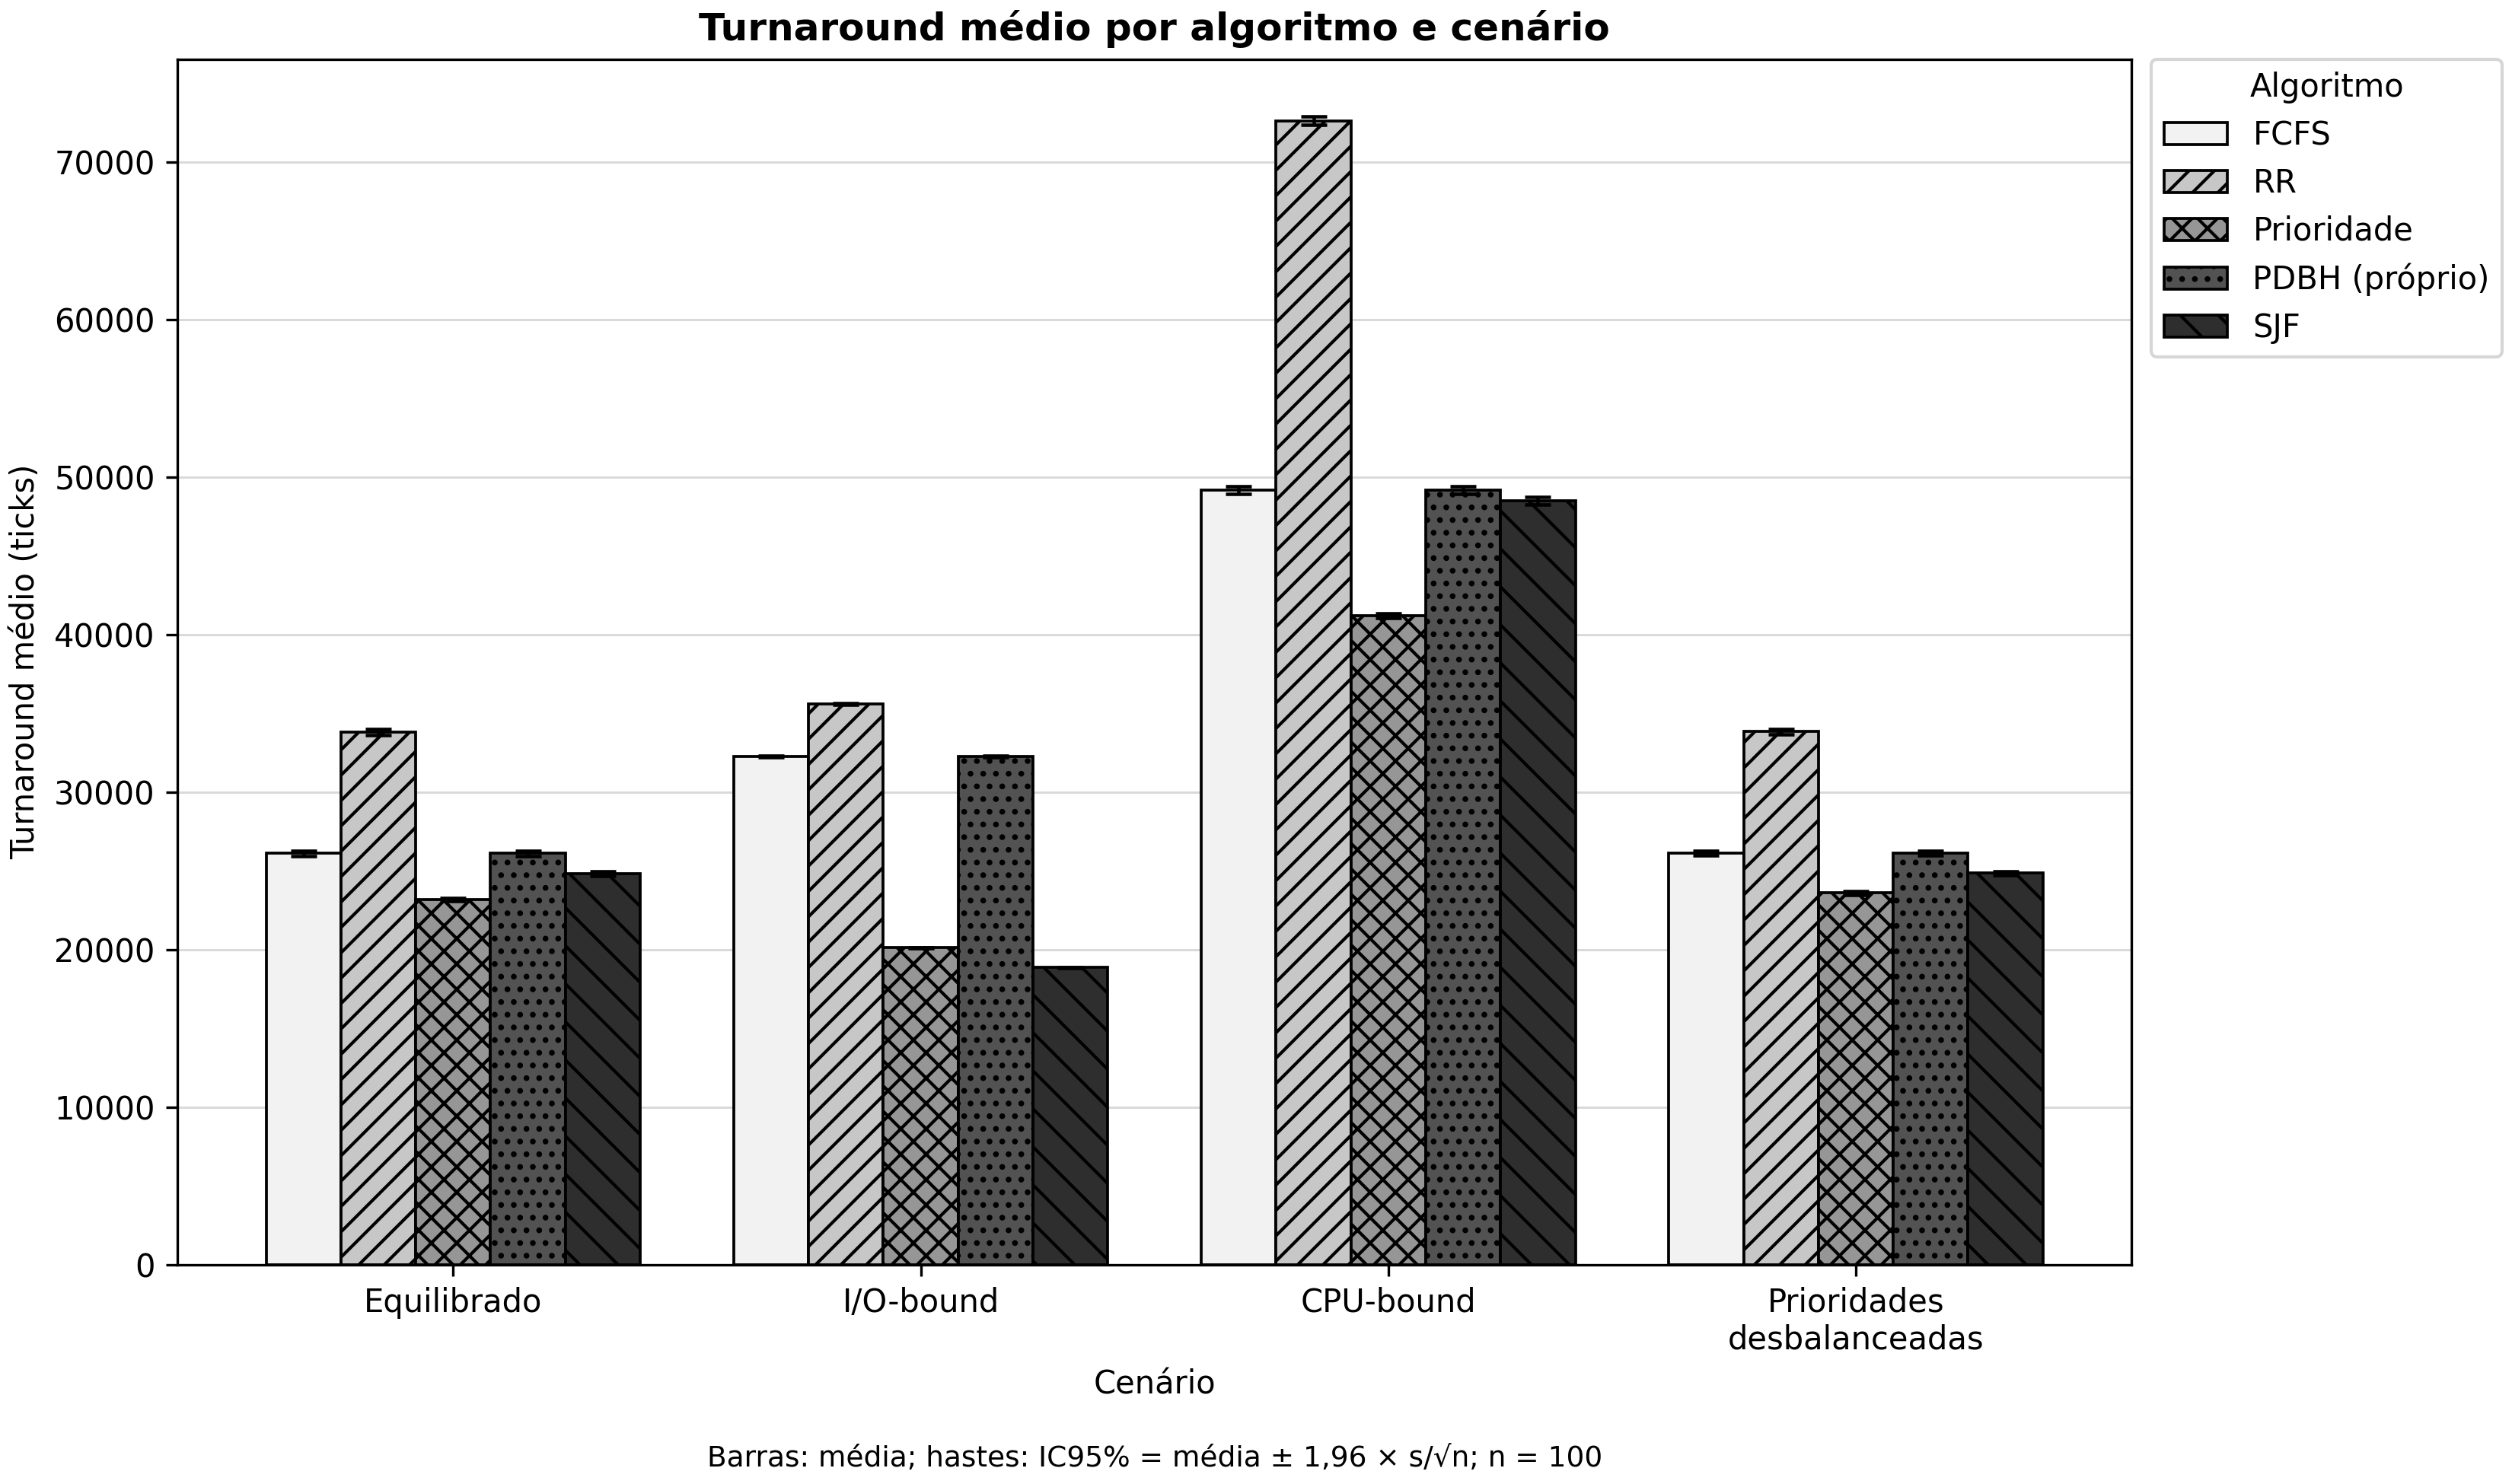
\includegraphics[width=\linewidth]{../results/figures/mean_turnaround_ic95.png}}
\caption{Turnaround médio com IC95\% (unidade: ticks).}
\label{fig:turnaround}
\end{figure}

\begin{figure}[htbp]
\centerline{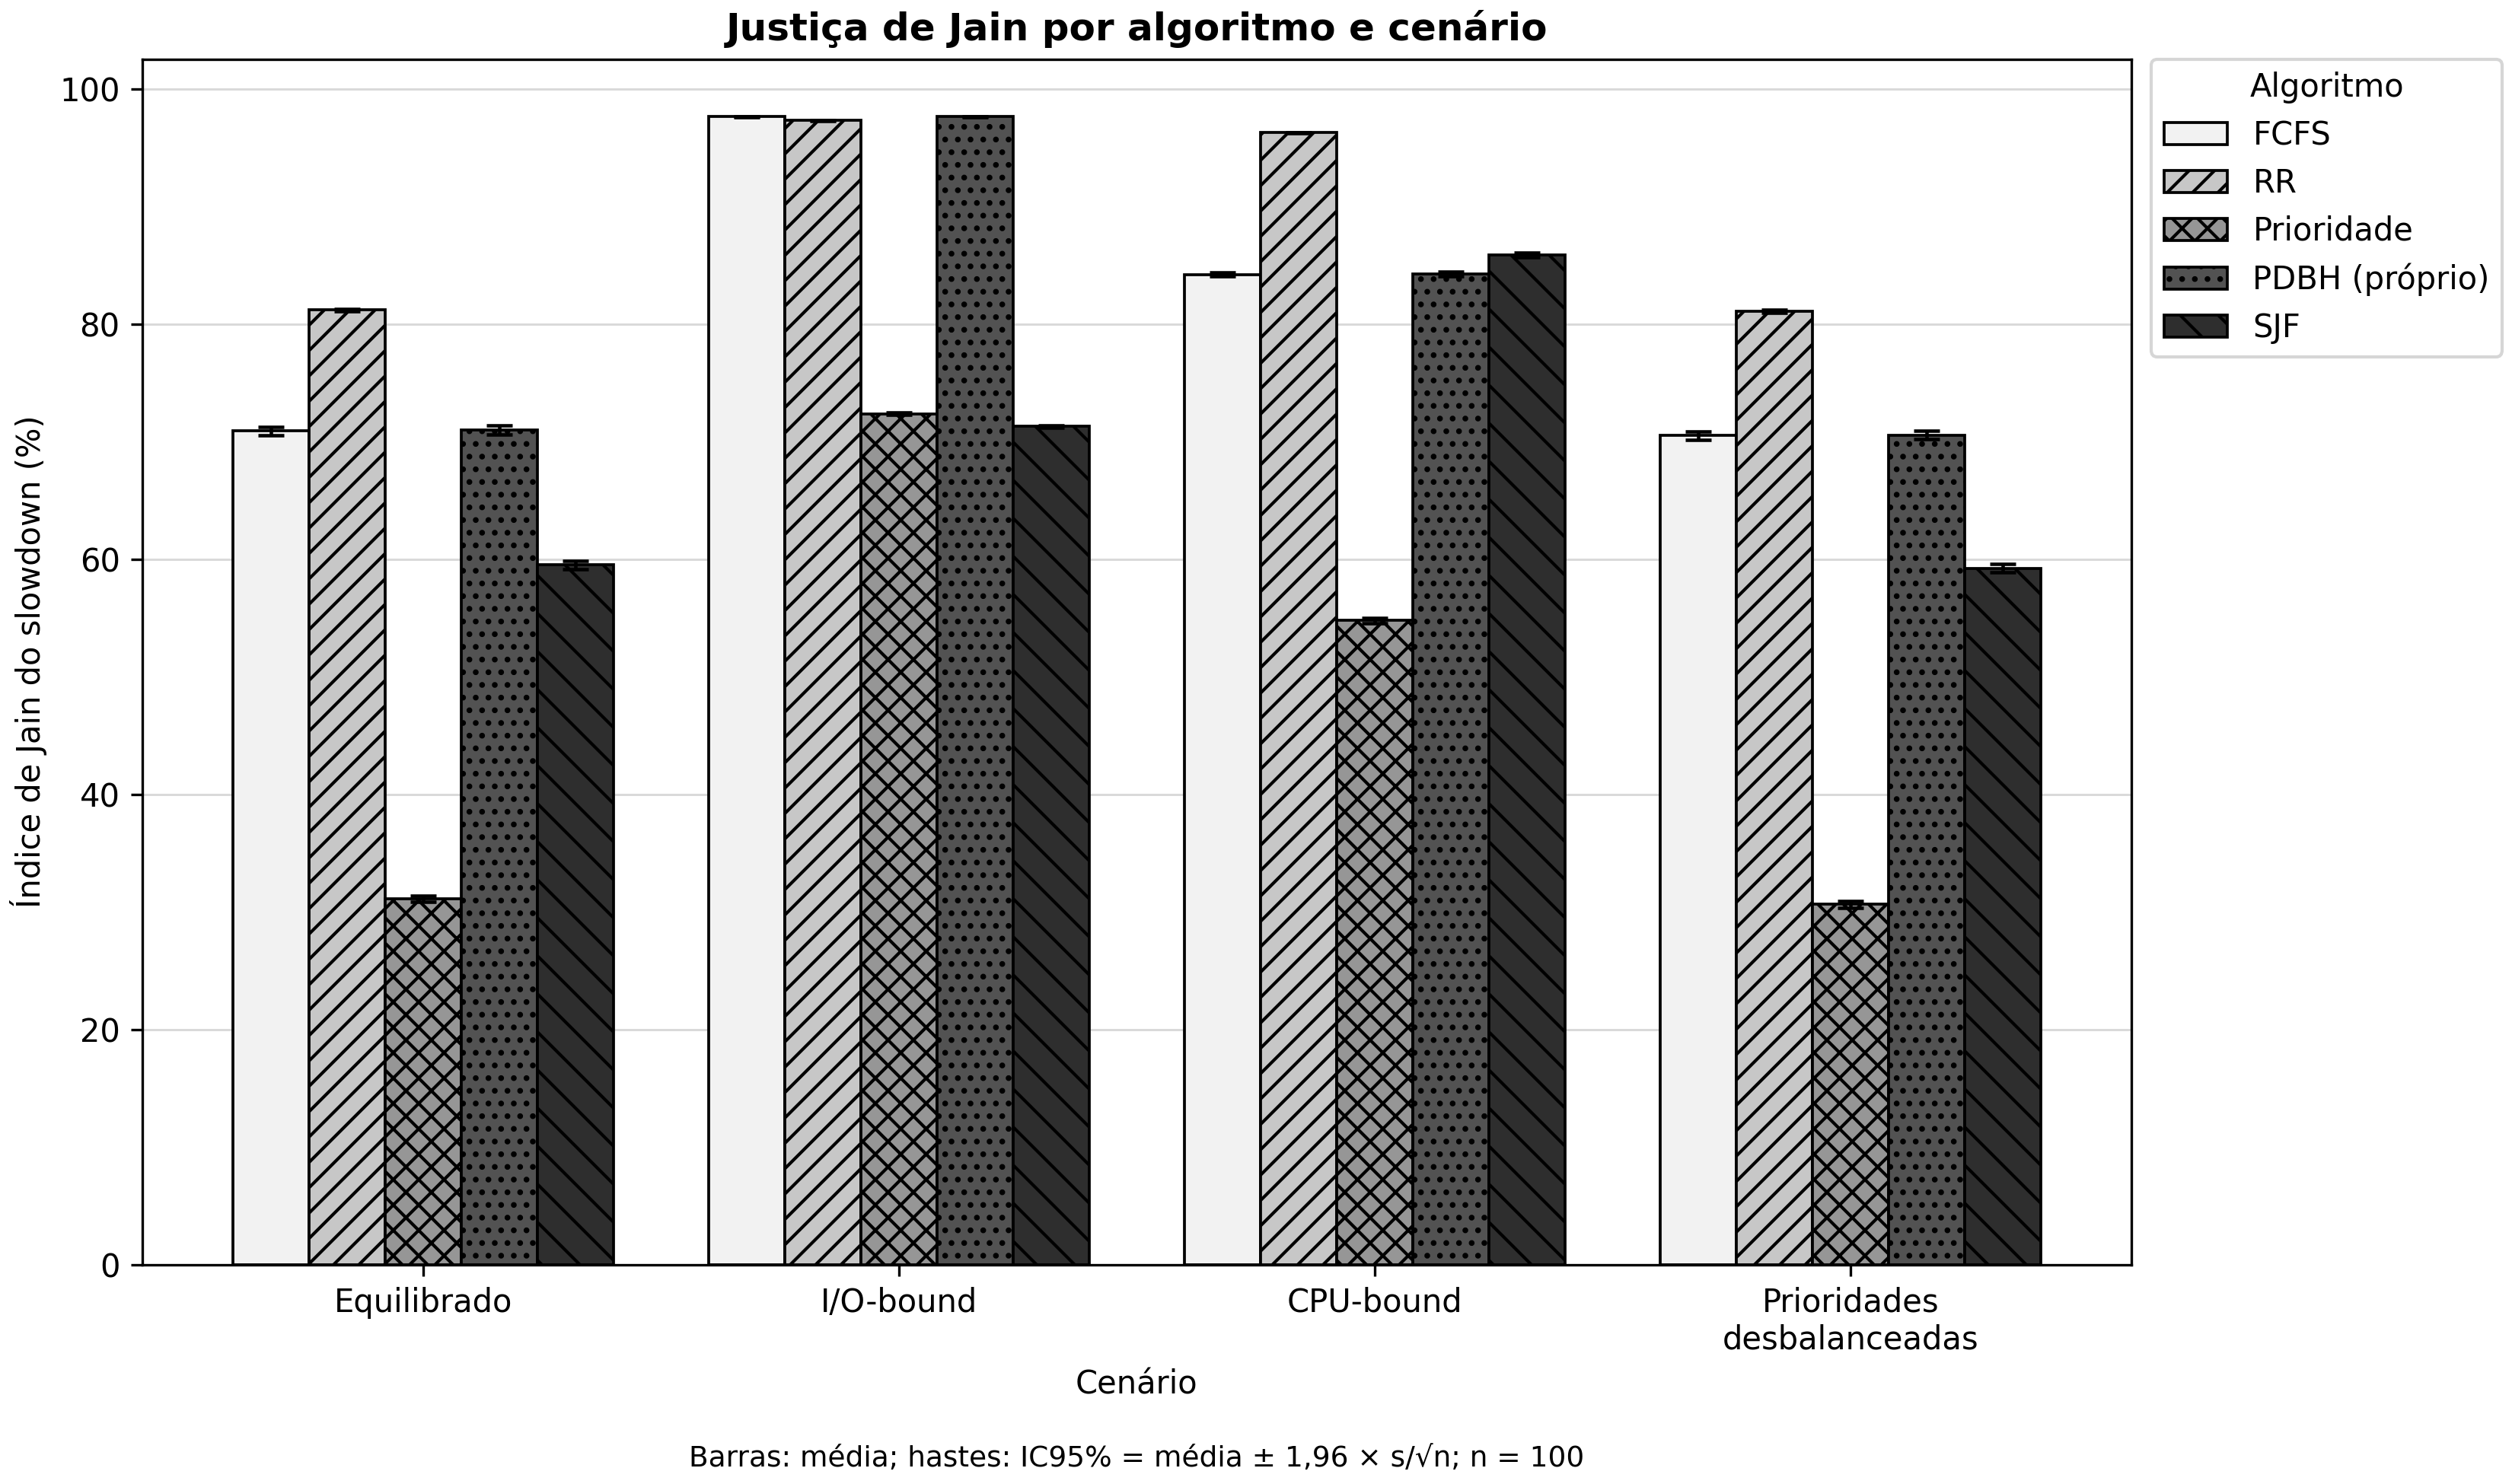
\includegraphics[width=\linewidth]{../results/figures/jain_slowdown_pct_ic95.png}}
\caption{Equidade: Índice de Jain do Slowdown com IC95\% (unidade: \%).}
\label{fig:jain}
\end{figure}

\begin{figure}[htbp]
\centerline{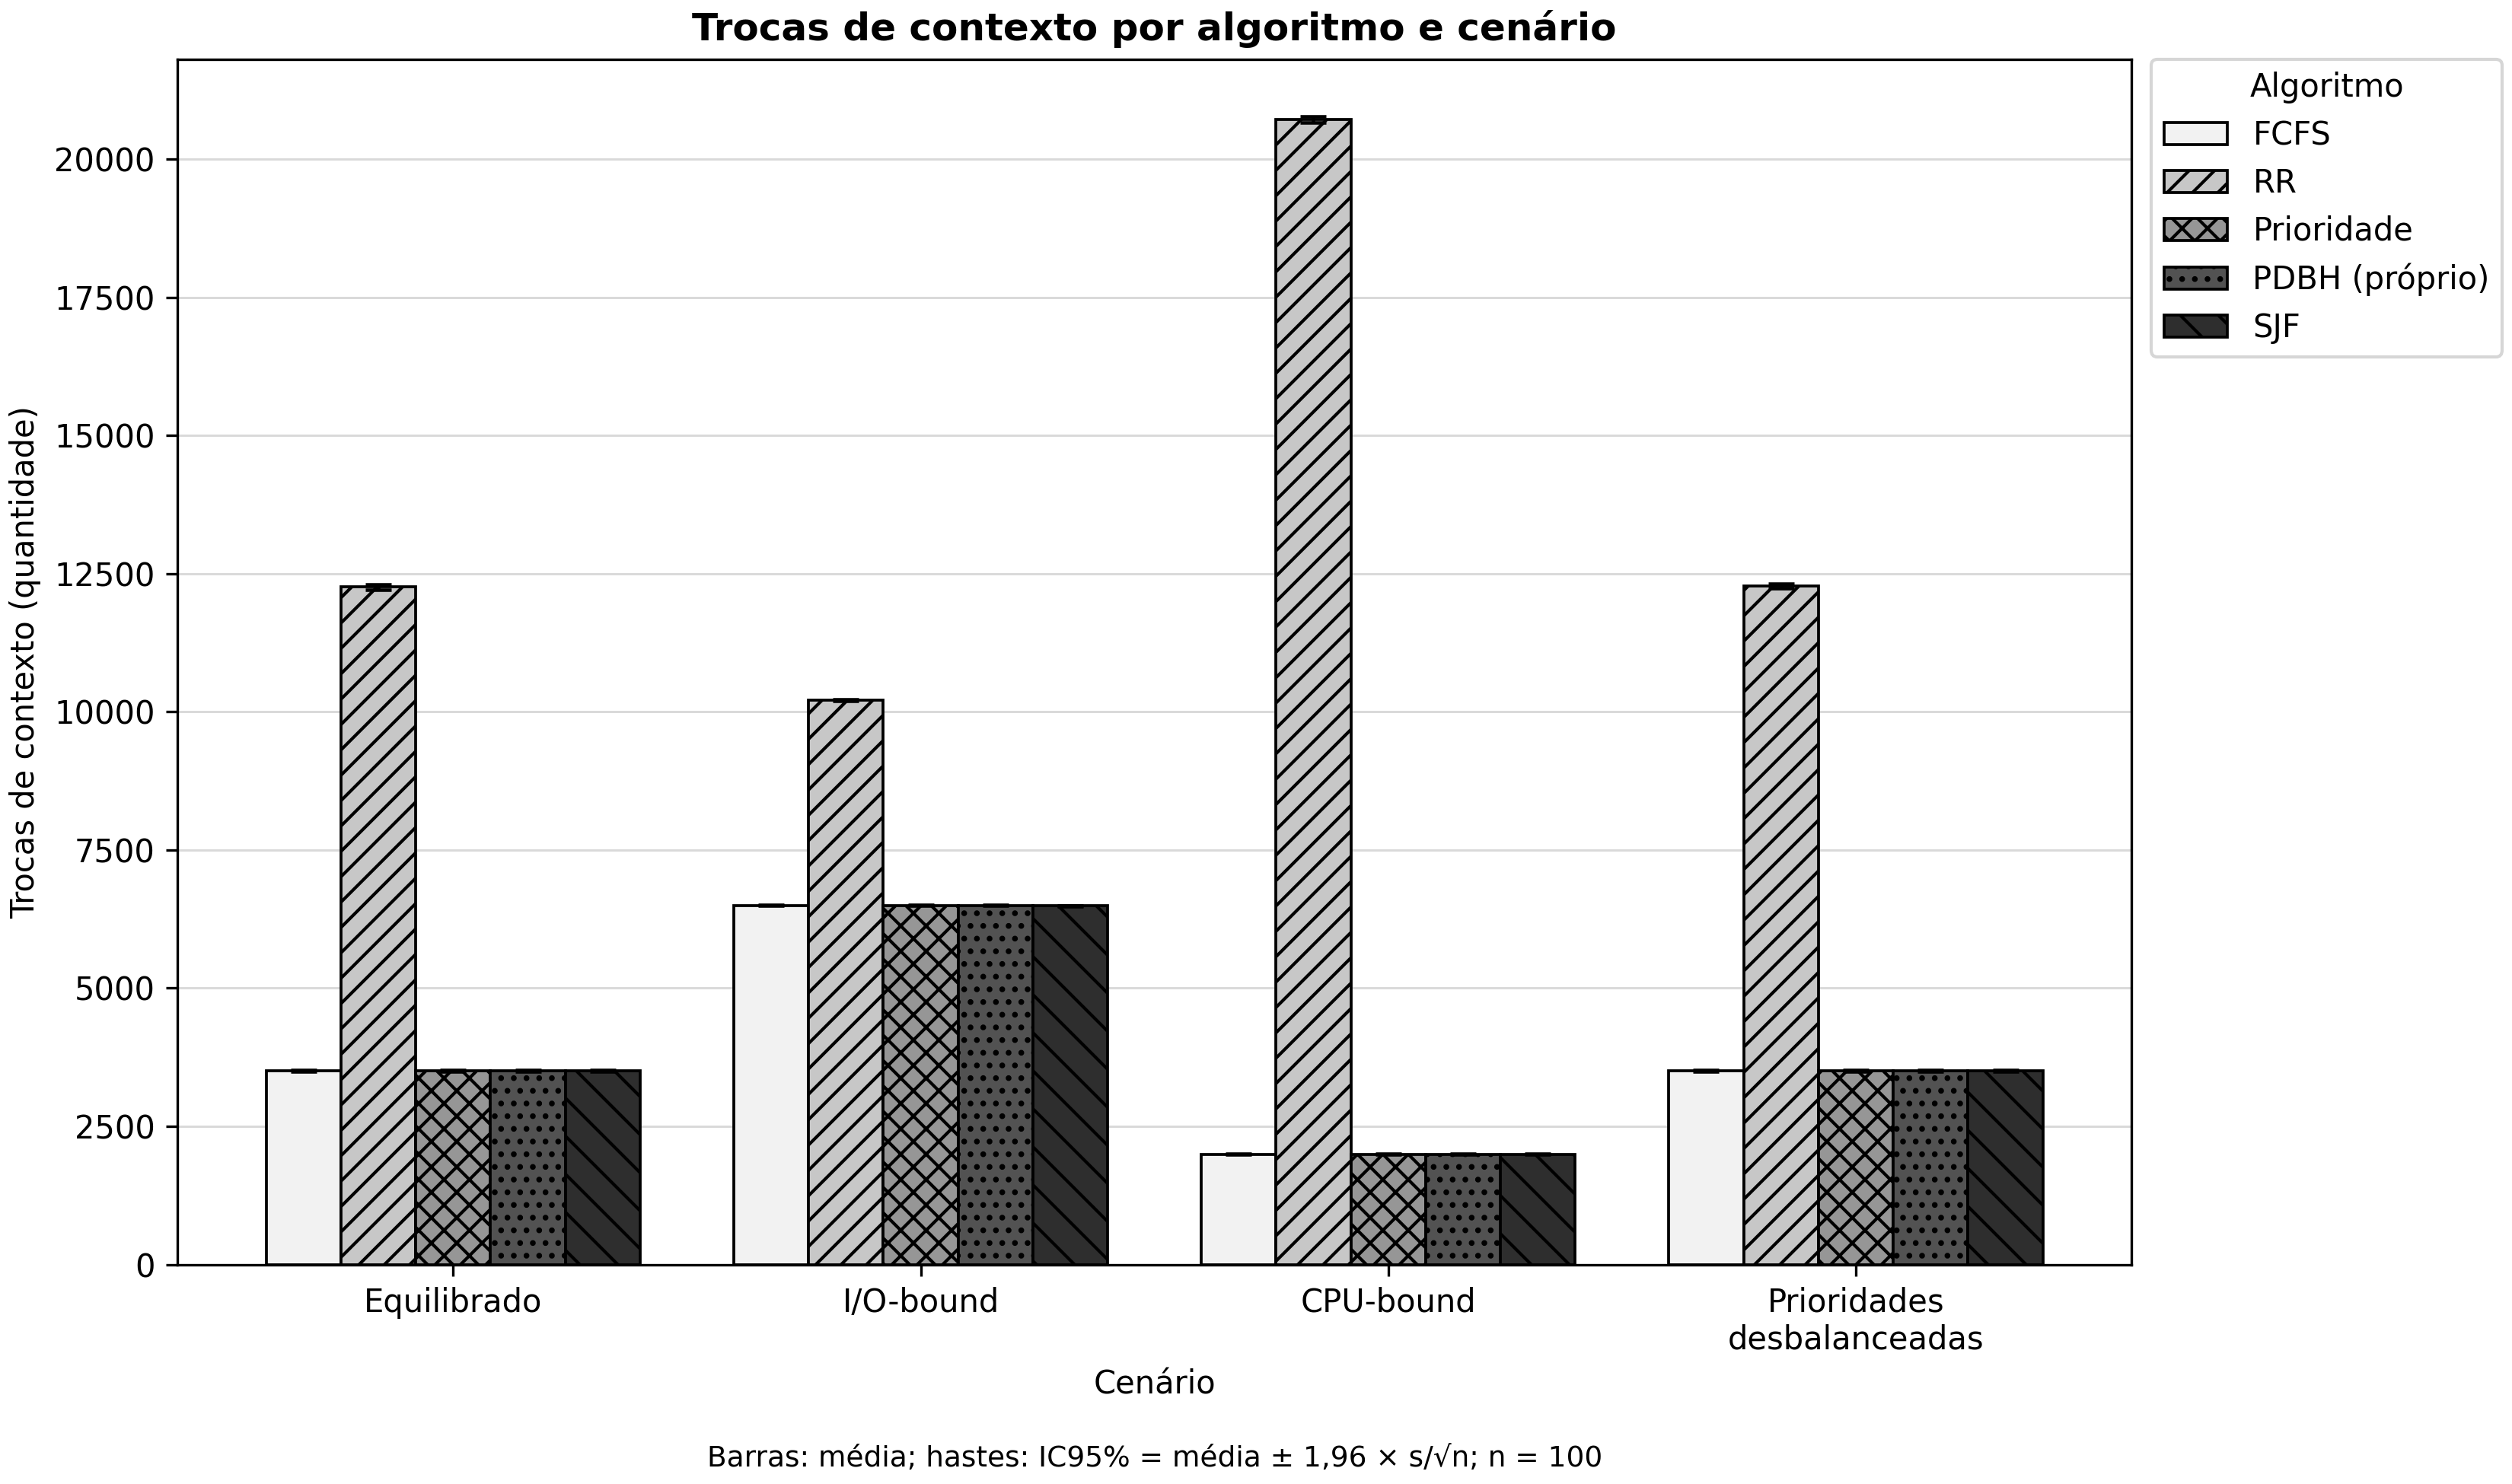
\includegraphics[width=\linewidth]{../results/figures/context_switches_ic95.png}}
\caption{Custo Sistêmico: Trocas de Contexto com IC95\% (unidade: ocorrências).}
\label{fig:context}
\end{figure}

\subsection{Cenário: Equilibrado}
No cenário equilibrado, os resultados para a métrica de Turnaround Médio (em ticks) foram:
\begin{itemize}
    \item FCFS: 26.112,67 [IC95\%: 25.948,63 -- 26.276,72]
    \item Round Robin: 33.817,33 [IC95\%: 33.624,15 -- 34.010,51]
    \item Prioridade: 23.189,82 [IC95\%: 23.083,25 -- 23.296,40]
    \item PDBH (Proposto): 26.112,71 [IC95\%: 25.949,17 -- 26.276,25]
\end{itemize}

Para a métrica de Equidade (Índice de Jain do Slowdown):
\begin{itemize}
    \item FCFS: 70,91\% [IC95\%: 70,53\% -- 71,28\%]
    \item Round Robin: 81,21\% [IC95\%: 81,09\% -- 81,32\%]
    \item Prioridade: 31,10\% [IC95\%: 30,86\% -- 31,34\%]
    \item PDBH (Proposto): 70,99\% [IC95\%: 70,62\% -- 71,37\%]
\end{itemize}

O volume de Trocas de Contexto acompanhou a natureza preemptiva das políticas. O Round Robin contabilizou 12.260 trocas [IC95\%: 12.213,18 -- 12.308,61], enquanto os demais algoritmos (FCFS, Prioridade e PDBH) apresentaram exatamente 3.504,90 trocas [IC95\%: 3.491,50 -- 3.518,29].

\subsection{Cenário: I/O-Bound}
No cenário de alta intensidade de Entrada/Saída (I/O-Bound), os resultados para a métrica de Turnaround Médio (em ticks) foram:
\begin{itemize}
    \item FCFS: 32.268,65 [IC95\%: 32.221,99 -- 32.315,31]
    \item Round Robin: 35.607,17 [IC95\%: 35.554,87 -- 35.659,47]
    \item Prioridade: 20.120,75 [IC95\%: 20.090,48 -- 20.151,02]
    \item PDBH (Proposto): 32.268,25 [IC95\%: 32.221,65 -- 32.314,84]
\end{itemize}

Para a métrica de Equidade (Índice de Jain do Slowdown):
\begin{itemize}
    \item FCFS: 97,66\% [IC95\%: 97,64\% -- 97,68\%]
    \item Round Robin: 97,32\% [IC95\%: 97,30\% -- 97,35\%]
    \item Prioridade: 72,38\% [IC95\%: 72,30\% -- 72,47\%]
    \item PDBH (Proposto): 97,65\% [IC95\%: 97,63\% -- 97,67\%]
\end{itemize}

O número de Trocas de Contexto acompanhou a fragmentação imposta pelo quantum no Round Robin, que contabilizou 10.212,15 trocas [IC95\%: 10.200,51 -- 10.223,79]. Os algoritmos não preemptivos registraram 6.498,87 trocas [IC95\%: 6.492,07 -- 6.505,67].

\subsection{Cenário: CPU-Bound}
Para o cenário CPU-Bound, caracterizado por rajadas longas de processamento e poucas requisições de E/S, os resultados para a métrica de Turnaround Médio (em ticks) foram:
\begin{itemize}
    \item FCFS: 49.180,78 [IC95\%: 48.949,41 -- 49.412,14]
    \item Round Robin: 72.641,57 [IC95\%: 72.367,75 -- 72.915,38]
    \item Prioridade: 41.199,78 [IC95\%: 41.054,63 -- 41.344,94]
    \item PDBH (Proposto): 49.192,65 [IC95\%: 48.959,46 -- 49.425,84]
\end{itemize}

Para a métrica de Equidade (Índice de Jain do Slowdown):
\begin{itemize}
    \item FCFS: 84,22\% [IC95\%: 84,06\% -- 84,39\%]
    \item Round Robin: 96,29\% [IC95\%: 96,26\% -- 96,32\%]
    \item Prioridade: 54,79\% [IC95\%: 54,56\% -- 55,02\%]
    \item PDBH (Proposto): 84,26\% [IC95\%: 84,09\% -- 84,44\%]
\end{itemize}

As Trocas de Contexto refletiram a retenção da CPU: o Round Robin atingiu 20.714,96 trocas [IC95\%: 20.658,90 -- 20.771,01], enquanto os algoritmos não preemptivos registraram 1.996,75 trocas [IC95\%: 1.991,98 -- 2.001,51].

\subsection{Cenário: Desbalanceado (70\% Alta Prioridade)}
Neste cenário, onde a grande maioria dos processos chega com prioridade estática alta, os resultados para o Turnaround Médio (em ticks) foram:
\begin{itemize}
    \item FCFS: 26.120,46 [IC95\%: 25.969,06 -- 26.271,86]
    \item Round Robin: 33.841,36 [IC95\%: 33.663,37 -- 34.019,35]
    \item Prioridade: 23.596,96 [IC95\%: 23.491,27 -- 23.702,64]
    \item PDBH (Proposto): 26.120,99 [IC95\%: 25.970,05 -- 26.271,92]
\end{itemize}

Para a métrica de Equidade (Índice de Jain do Slowdown):
\begin{itemize}
    \item FCFS: 70,51\% [IC95\%: 70,14\% -- 70,88\%]
    \item Round Robin: 81,09\% [IC95\%: 80,97\% -- 81,20\%]
    \item Prioridade: 30,65\% [IC95\%: 30,37\% -- 30,93\%]
    \item PDBH (Proposto): 70,57\% [IC95\%: 70,20\% -- 70,94\%]
\end{itemize}

As Trocas de Contexto mantiveram o padrão dos cenários anteriores: 12.272,37 trocas para o Round Robin [IC95\%: 12.228,45 -- 12.316,28] e exatas 3.508,79 trocas para as políticas não preemptivas [IC95\%: 3.496,66 -- 3.520,91].

\section{Discussão e Análise do Algoritmo PDBH}
A análise estatística dos quatro cenários evidencia as dinâmicas de \textit{trade-off} estabelecidas. A política de Prioridade Estática sempre obteve os menores Tempos de Turnaround absolutos, beneficiando-se da retenção de processos-chave. Entretanto, o custo sistêmico desse benefício foi a queda brusca na equidade, com o Índice de Jain despencando para a faixa de 30\% a 72\%, indicando uma forte tendência ao estado de inanição (\textit{starvation}) para processos menos favorecidos, especialmente no cenário Desbalanceado.

O Round Robin, em contraste, obteve os maiores Índices de Jain (acima de 80\% e até 97\% em I/O-Bound), porém penalizou muito o Turnaround. Esta queda no desempenho é explicada pela própria estrutura do fatiamento sistemático do \textit{quantum}, cujo impacto triplica a ocorrência de trocas de contexto, como demonstrado pelos dados de CPU-Bound (mais de 20.700 trocas).

\textbf{Análise sobre o algoritmo próprio (PDBH)}

Em relação ao algoritmo desenvolvido pela equipe (PDBH), o projeto buscou diminuir os problemas de inanição da prioridade estática enquanto recompensa a espera em fila. Entretanto, comparado aos algoritmos clássicos obrigatórios, \textbf{o PDBH não obteve melhor desempenho em nenhum cenário e não gerou melhora em nenhuma métrica}. Ao contrário, apresentou sobreposição estatística completa de seus Intervalos de Confiança (IC95\%) com o algoritmo FCFS, indicando comportamento idêntico em Turnaround, Equidade e Trocas de Contexto. 

Diferente do esperado, a política também exibiu seu \textbf{pior desempenho (relativo)} no cenário CPU-Bound, onde registrou uma piora de equidade (Jain de 84,26\%) quando comparada ao modelo Round Robin (96,29\%), sem ser capaz de contornar a monopolização da CPU.

O principal \textbf{custo introduzido} pelo PDBH não se refletiu em um aumento de trocas de contexto (já que sua taxa acompanhou a do FCFS, em torno de 3.500 trocas em cenários equilibrados), mas sim num alto peso (\textit{overhead}) de complexidade. Por demandar o recálculo da pontuação a cada ponto de despacho considerando o tempo atual, o PDBH requer uma varredura $O(N)$ em toda a fila de prontos, injetando processamento extra.

\textbf{Por que esses resultados aconteceram?}

Os resultados espelhados ao FCFS decorrem exclusivamente da limitação da arquitetura do PDBH: \textbf{a ausência de preempção}. 
Em um cenário CPU-Bound, enquanto uma tarefa longa monopoliza o processador, todos os demais processos aguardando na fila acumulam bônus de espera ativa simultaneamente. Ao fim da rajada, quando a CPU é finalmente devolvida, o processo com maior tempo de chegada naturalmente acumulou a maior quantidade de bônus na fórmula. O nivelamento do envelhecimento faz com que os pesos da fórmula não tenham efeito e transforma o algoritmo em um espelho direto do FCFS. No cenário I/O-Bound, o oposto ocorreu: frequentes bloqueios de E/S reiniciavam constantemente o relógio de espera dos processos ($ready\_since$), impedindo-os de alcançar os limites mínimos de acúmulo de bônus, fazendo a fórmula retornar, novamente, às posições naturais de ordem de chegada do FCFS.

\section{Conclusão}
A execução das simulações comprovou matematicamente a dependência entre métricas e cenários para as políticas clássicas. A política de Prioridade obteve o menor Turnaround médio em todos os contextos, porém sua dificuldade em garantir equidade a torna ruim para cargas densas, gerando muita inanição (como mostra o baixo Índice de Jain). O Round Robin resolve bem a falta de justiça no acesso à CPU, confirmada por valores altos de Jain, mas prejudica bastante o Tempo de Retorno (\textit{Turnaround}) por injetar enormes volumes de Trocas de Contexto devido às interrupções temporais.

Ao comparar o algoritmo próprio (PDBH) com os algoritmos clássicos (FCFS, RR, Prioridade Estática e SJF), conclui-se que o uso isolado de pontuações dinâmicas de histórico em arquiteturas não preemptivas não funciona na prática. Independente das penalidades (por CPU) ou bônus (por espera) propostos, os resultados comprovaram estatisticamente que a fórmula acaba voltando para a ordem de chegada (FCFS) em todos os cenários e métricas analisadas. O PDBH falhou em melhorar a justiça ou o Turnaround porque o envelhecimento cumulativo da fila, sem um mecanismo para interromper de imediato quem monopoliza o processador, anula suas próprias regras e adiciona apenas custo operacional sistêmico.

\begin{thebibliography}{00}
\bibitem{silberschatz}
Silberschatz, A., Galvin, P. B., e Gagne, G.
\newblock Sistemas Operacionais com Java.
\newblock Elsevier, 2015.
\end{thebibliography}

\end{document}
